
\section{View\label{sec:ImplementationView}}

As the view our engine provides is only a framework for making an
actual view, it limits what can be said about its implementation.
What this section will focus on is why we chose to design the view
in this manner and how we provide ways to ensure that the view can
be executed on a different thread while not being affected by its
problems.

\begin{figure}
\begin{centering}
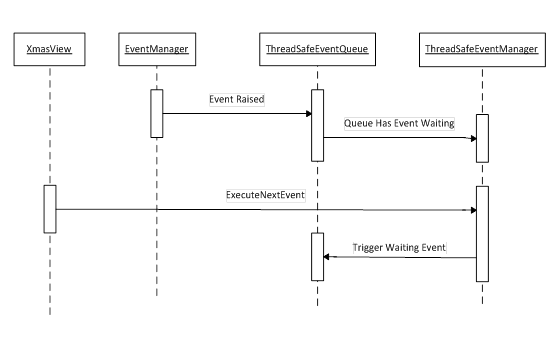
\includegraphics[width=0.7\textwidth]{ViewImpThreadSafeSequenceDiagram}
\par\end{centering}

\caption{Sequence diagram show how events triggered on the model is stored
and put on hold until the view thread is able to process them\label{fig:ThreadSafeSequenceDiagram}}
\end{figure}



\subsection*{Design}

The view design for the engine was never meant to be an actual view,
this would limit the potential of what could be done so we are rather
content with not providing more than the skeleton for making a proper
view. The idea is that the actual implementation of a view should
be part of some extension to make a view that displays graphics or
a view that shows a console, it should never be a core part of the
engine. The core engine should only provide what all views need, this
means that if just a single view is restricted by our design then
our design is flawed.


\subsection*{Thread Safety}

One thing all views have in common is the dangers of having code that
is not thread safe, by having two threads run through the same address
space at the same time, the guarantee of a race condition or deadlock
is very high. This makes programming a view rather difficult. To combat
this problem, we came up with the \texttt{ThreadSafeEventManager}
and the \texttt{ThreadSafeEventQueue}. These classes both assist with
ensuring that the model thread is never involved in the view thread\textquoteright{}s
business. The way the \texttt{ThreadSafeEventManager} works is by
storing all events triggered by the EventManager of the model, the
events data are all kept safe and the order in which the events was
triggered is also kept. The idea is that when the view thread is not
performing any actions, such as when it is in sleep mode between a
draw update, instead of sleeping it will call the \texttt{ThreadSafeEventManager}
and tell it to begin executing. The process works by running the \texttt{ThreadSafeEventQueue}
that had one of its events trigger and tell it to execute. When all
\texttt{ThreadSafeEventQueue} are empty then that mean that there
are no longer any events waiting to be executed on the view thread.
Since views are only interested in seeing the changes to the world
and not how the changes came about, then that means that the views
only need access to the events and not the actions. To see a sequence
diagram of this process look at fig. \ref{fig:ThreadSafeSequenceDiagram}.


\subsection*{Summary}

The view design is mostly focused on ensuring that the user of the
engine should deal with as few threading problems as possible as such
we have developed two classes \texttt{ThreadSafeEventQueue} and \texttt{ThreadSafeEventManager}
these both make it possible for the view to trigger events when the
thread is free from other duties, instead of relying on the model
thread to also handle view event updates. 
